\documentclass{../source/Experiment}

\major{信息工程}
\name{姚桂涛}
\title{幅度调制与解调}
\expname{幅度调制与解调}
\stuid{3190102932}
\college{信息与电子工程学院}
\date{\today}
\lab{东4-319}
\course{通信原理实验}
\instructor{金向东、龚淑君}
\grades{}
\exptype{验证性实验}
\partner{叶慷鹏}
\begin{document}
\makecover
\makeheader


\section{实验目的和要求}
    (1) 掌握幅度调制的原理和实现方法
    (2) 对调幅波信号的时域、频域特性进行测量分析
    (3) 掌握包络检波、同步检波的实现方法
    (4) 对解调输出信号进行测量分析

    \section{实验电路分析}

    AM、DSB调制实验电路如图3.6. 3所示。使用芯片MC1496实现两输入信号的乘法功能,    JP3端口输入高频载波信号,JP2端输入音频调制信号。AM幅度调制信号从JP4端输出,通过J3    跳线可以选取正向或负相已调信号的输出。在JP3端输入高频载波信号,调节定位器WR1,使    JP4端输出的载波信号幅度最小,再在JP2端输入音频调制信号,则JP4端输出抑制载波的幅度调    制信号DSB。

    \begin{figure}[H]
        \centering
        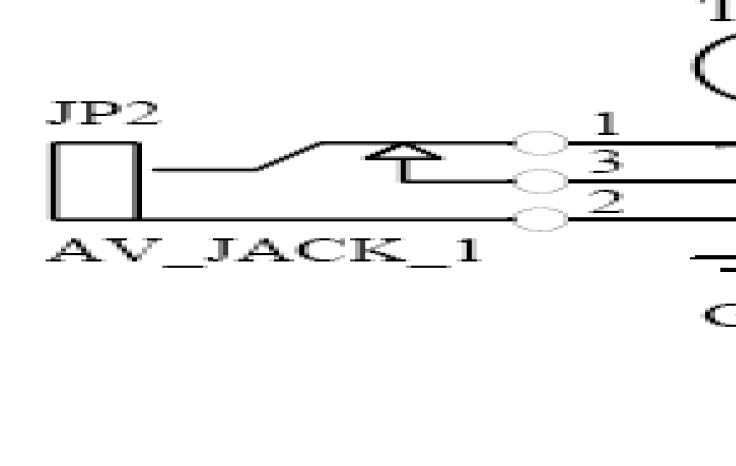
\includegraphics[width = 0.8\textwidth]{lab6-1}
        \caption{AM、DSB 调制电路}
    \end{figure}

    包络检波实验电路如图3.6. 4所示。输入信号由外部信号源在JP4端提供,接通跳线J5,将    信号送到检波电路中。为避免实验板上其它部分电路对包络检波电路的影响,跳线J3、J4要断    开。在TP8端口可以观察包络检波输出。另外,通过改变J1的跳线方式,选择不同的直流电阻阻值,改变滤波电路的时间常数,可在TP8端观察惰性失真情况;通过改变J2的跳线方式,改    变音频交流负载的阻抗值,在TP10端可观察负峰切割失真情况。

    \begin{figure}[H]
        \centering
        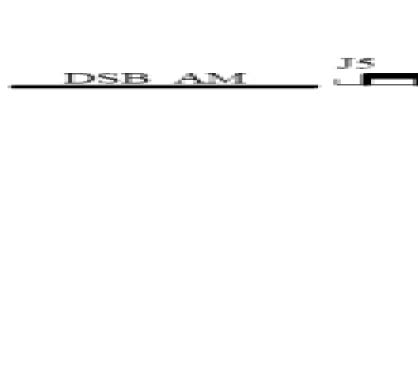
\includegraphics[width = 0.8\textwidth]{lab6-2}
        \caption{包络检波电路}
    \end{figure}
    
    同步相干解调实验电路如图3.6. 5所示,使用调制、解调芯片MC1496实现两输入信号的    乘法功能。本地载波信号与幅度调制时的载波信号是同一个信号,接通跳线J4,幅度调制信号    直接从电路板调制电路中获得。此时,为避免电路间的干扰,跳线J5要断开。经过滤波后的解    调输出信号从JP6端输出。

    \begin{figure}[H]
        \centering
        
\includegraphics[width = 0.8\textwidth]{lab6-3}
        \caption{包络检波电路}
    \end{figure}

    \section{实验数据与结果分析}
        \subsection{幅度调制实验}
            \subsubsection{普通幅度调制(AM)}
            JP3端由高频信号源输入频率为465kHz,大小为0dBm的正弦波作为载波信号输入;JP2端
            由信号源输入频率为1kHz,大小为0dBm的正弦波作为调制信号;接通跳线J3的1、2端或者2、
            3端;将平衡调节电位器WR1逆时针或顺时针旋到底。
            
            此次实验我们采用时域法调制度测量。

            用示波器观察调制输出信号波形(注意,示波器观察时将频谱分析仪的电缆从JP4脱开,
            避免信号被衰减):双通道观测,以JP2端输入的调制信号为示波器的触发源,观察调制输出
            TP4波形,测量其调制度。改变调制信号幅度,或调节平衡调节电位器WR1,分别将调制度调
            整到30\%、50\%和100\%,记录相应波形。
            
            \subsubsection{双边带调制(DSB)}

            在普通幅度调制的基础上,调节电位器WR1,同时观察信号频谱,直到频谱中载波分量降到最低,这就实现抑制载波幅度调制(DSB)。用示波器观察并记录调制输出信号的波形(注意,将频谱分析仪的电缆从JP4脱开)。

        \subsection{同步相干解调实验}

        \subsubsection{AM 同步解调}

        调整WR1,使调制电路产生AM调制信号,用示波器观测同步解调输出信号。改变JP2端调制信号幅度,从而改变已调波信号的调制度,观察同步解调输出信号的幅度变化。

        \subsubsection{DSB 同步解调}
        
        调整WR1,使调制电路产生DSB调制信号,用示波器观测同步解调输出信号。改变JP2端调制信号幅度,观察同步解调输出信号的幅度变化。

        \subsection{包络检波实验}
        
        \subsubsection{包络检波信号的测量}
        
        由高频信号源从JP4端输入载波频率为465kHz,大小为10dBm(即2Vp-p),调制信号频率为1kHz的正弦波,调制度为30\%的AM调幅信号。

        (1) 改变跳线 J1,选择不同的时间常数,用示波器在测试点 TP8观察检波输出信号的惰性失真情况。

        (2) 改变跳线 J2,选择不同的交流阻抗,用示波器在测试点 TP10观察检波输出信号的负峰切割失真情况。
        
        (3) 在无失真的情况下,改变输入信号的调制度,观察对输出信号的影响(何时出现失真)?
\section{实验数据分析}
\subsection{幅度调制实验}

\subsubsection{普通幅度调制(AM)}
(1) 时域法调制度测量:
用示波器观察调制输出信号波形(注意,示波器观察时将频谱分析仪的电缆从JP4脱开,
避免信号被衰减):双通道观测,以JP2端输入的调制信号为示波器的触发源,观察调制输出
TP4波形,测量其调制度。改变调制信号幅度,或调节平衡调节电位器WR1,分别将调制度调
整到30\%、50\%和100\%,记录相应波形。

30\%时可以计算出$E_{\max }:E_{\min }$=1.857,其波形为:
\begin{figure}[H]
    \centering
    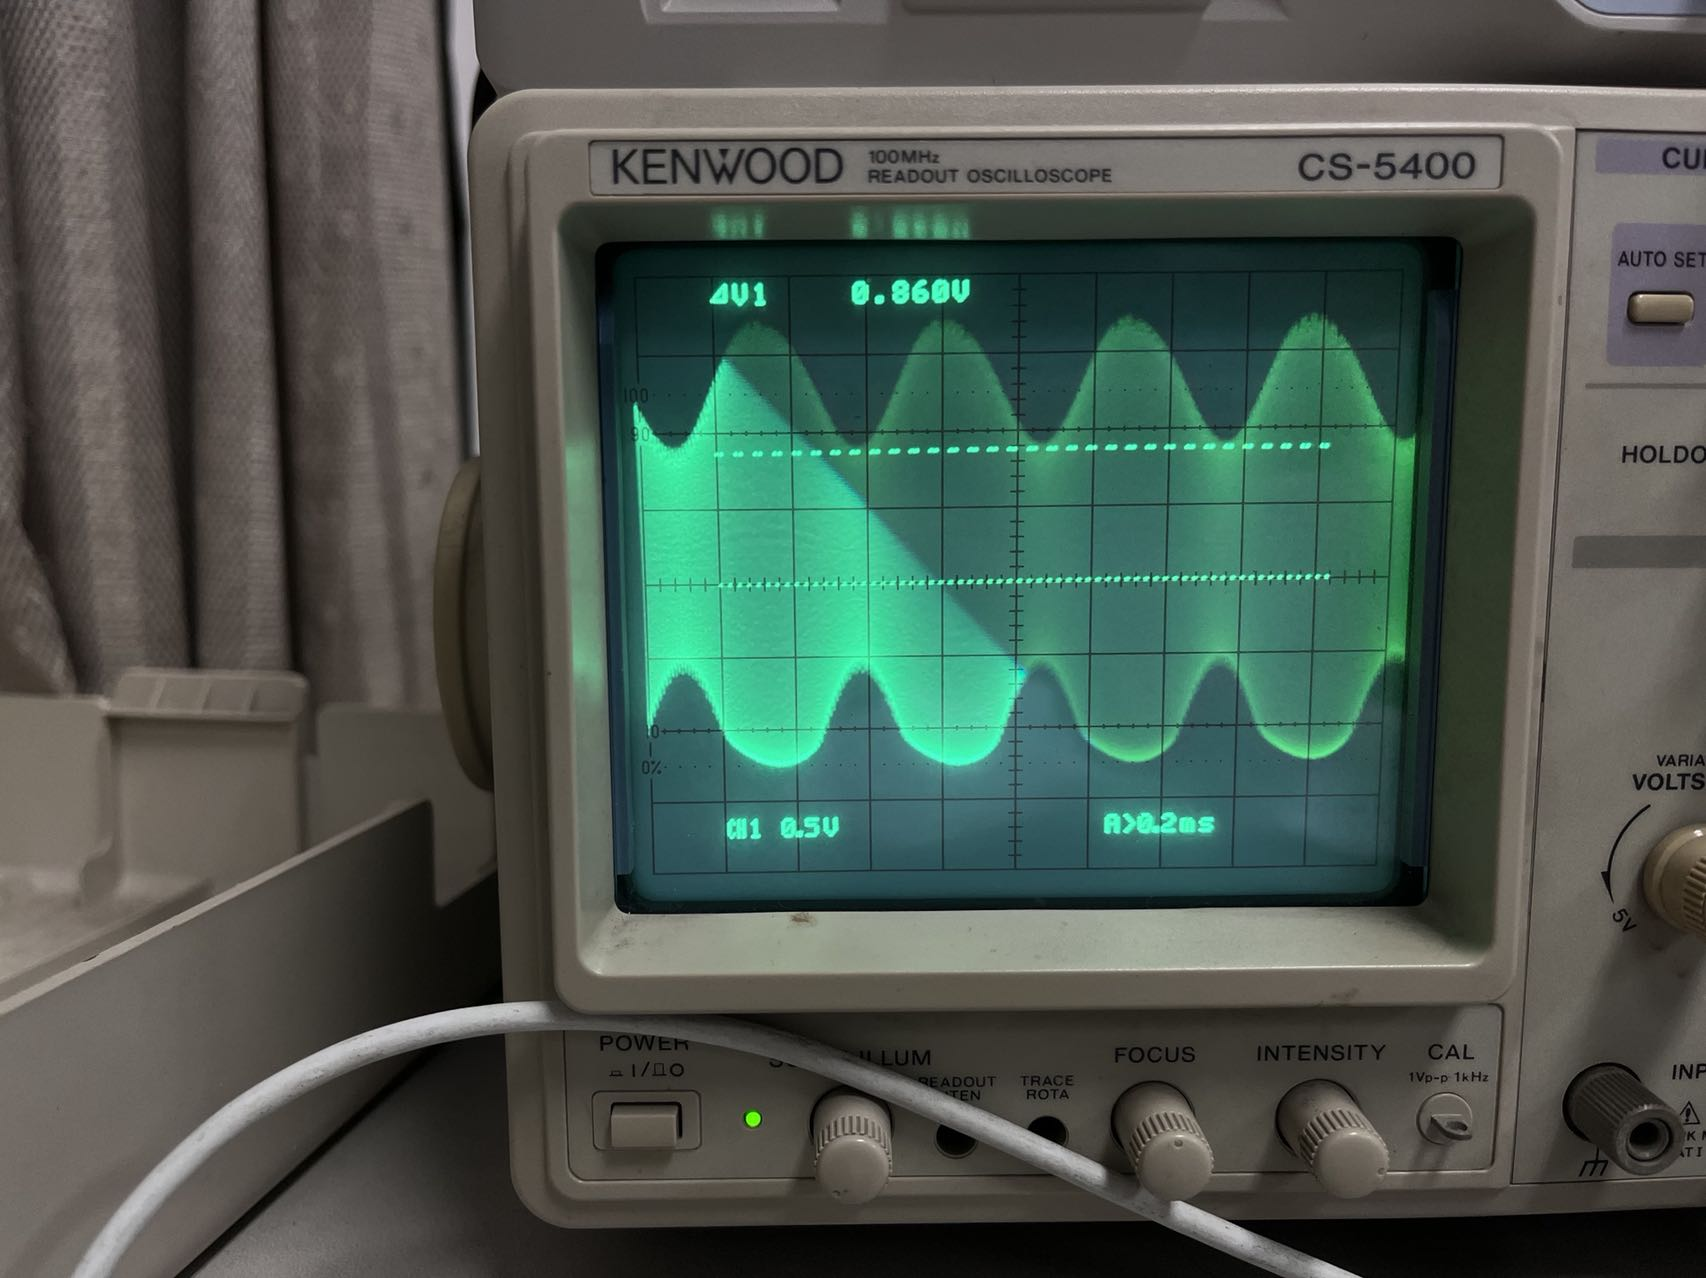
\includegraphics[width = 0.5\textwidth]{lab6/6.png}
    \caption{调制度30\%相应波形}
\end{figure}

50\%时可以计算出$E_{\max }:E_{\min }$=3,其波形为:
\begin{figure}[H]
    \centering
    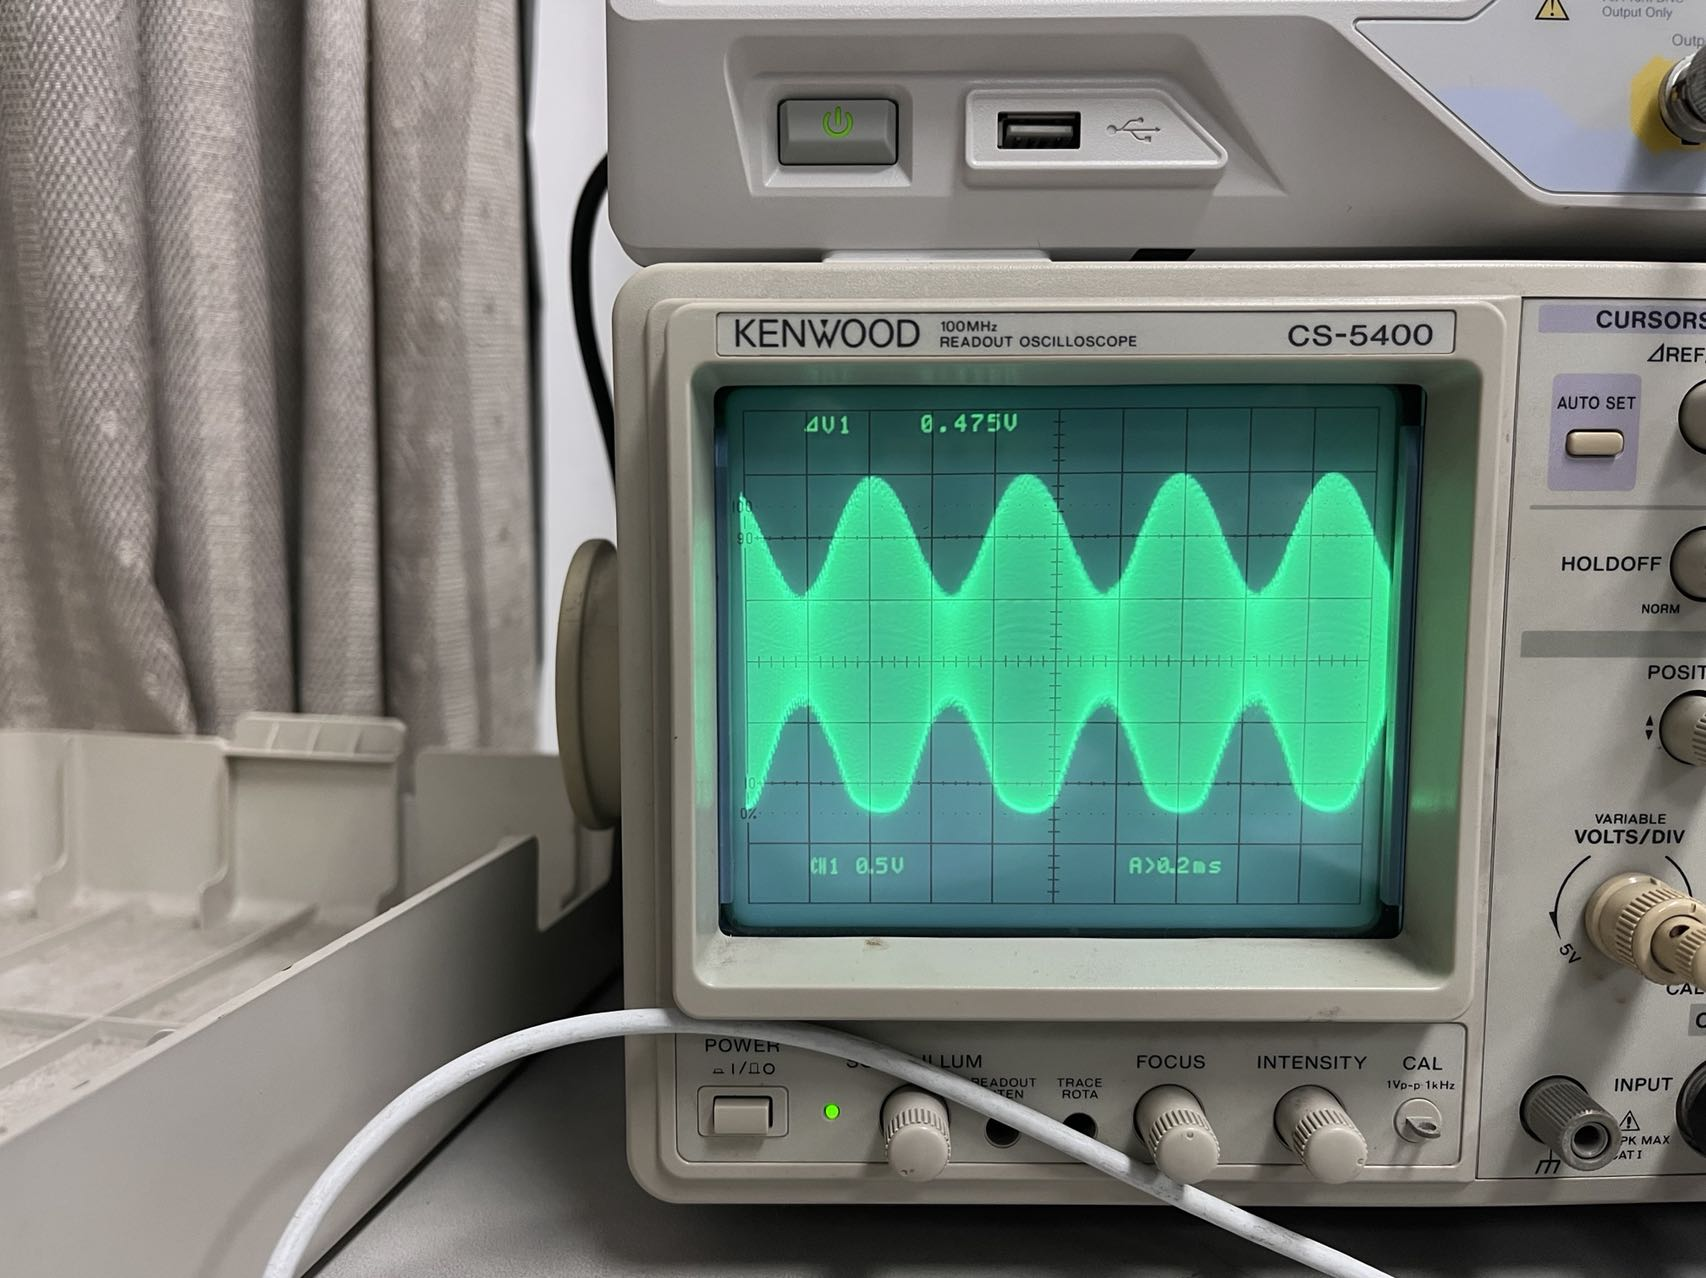
\includegraphics[width = 0.5\textwidth]{lab6/7.png}
    \caption{调制度50\%相应波形}
\end{figure}

100\%时$E_{\min }$=0即可,其波形为:
\begin{figure}[H]
    \centering
    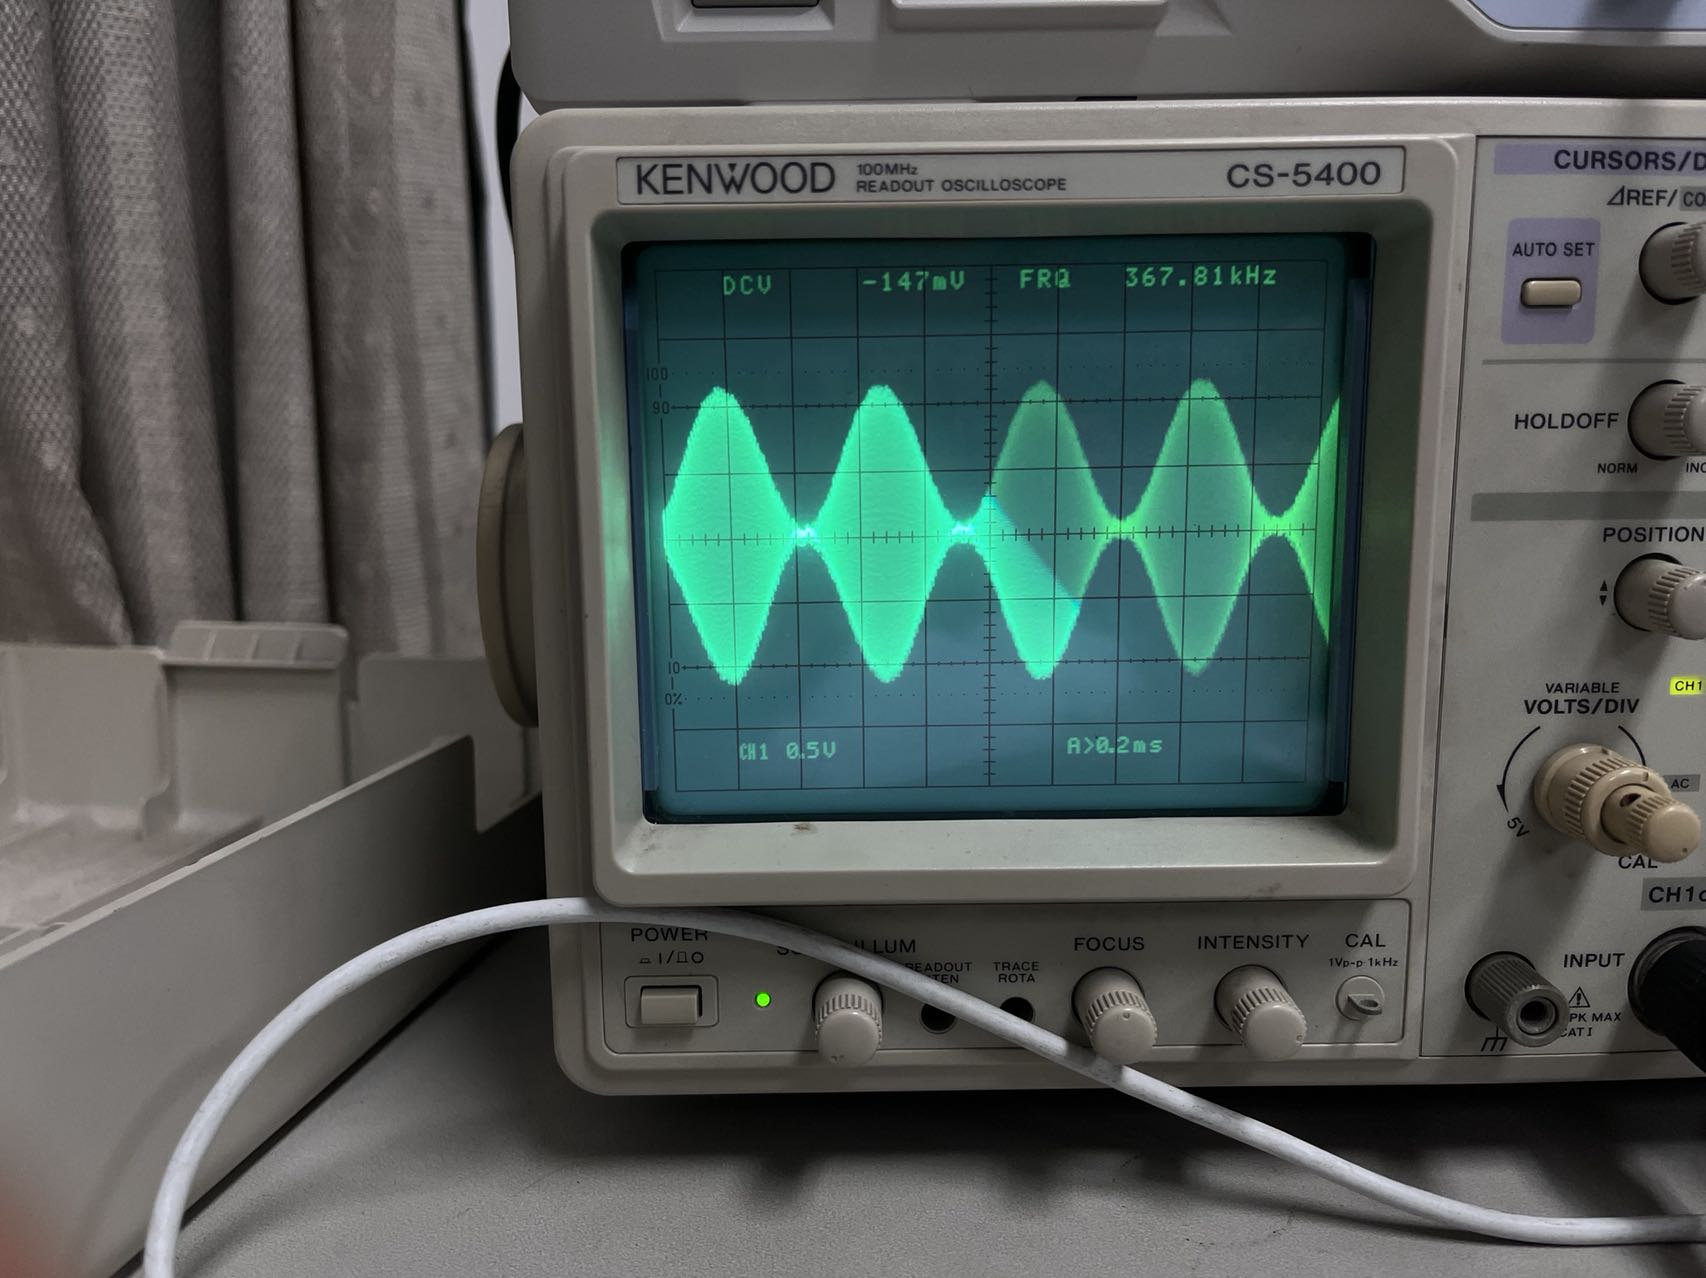
\includegraphics[width = 0.5\textwidth]{lab6/8.png}
    \caption{调制度100\%相应波形}
\end{figure}

可以看到调制度越高,$E_{\max }:E_{\min }$就越大。

(2) 频域法调制度测量:

AM 调制度也可以采用频谱分析法得到:当分辨率带宽设置为RBW <<$f_m$调制频率
时,
频谱分析仪可以观测到载波信号
$f_C$ 及相隔一个调制频率
$f_m$
的两个边带,调制度可由边带幅度和载波幅度的差值△
计算出来。

$\mathrm{m}=2 \times 10^{\Delta / 20} \times 100 \%$

将频谱分析仪的射频输入电缆连接调制输出接口 JP4;设定频谱分析仪的中心频率为
465kHz,扫描带宽为 10kHz,RBW 为 100Hz。观察调制输出信号的载波与上下边带频谱分量。
改变调制信号幅度,或调节平衡调节电位器 WR1,将边带与载波的幅度差△(可采用差值光
标法测量)分别调整为-16.5dBc、-12dBc 和-6dBc,分别计算相应的 AM 调制度。

第一次测量为边带与载波的幅度差△=-16.92dBc时:
\begin{figure}[H]
    \centering
    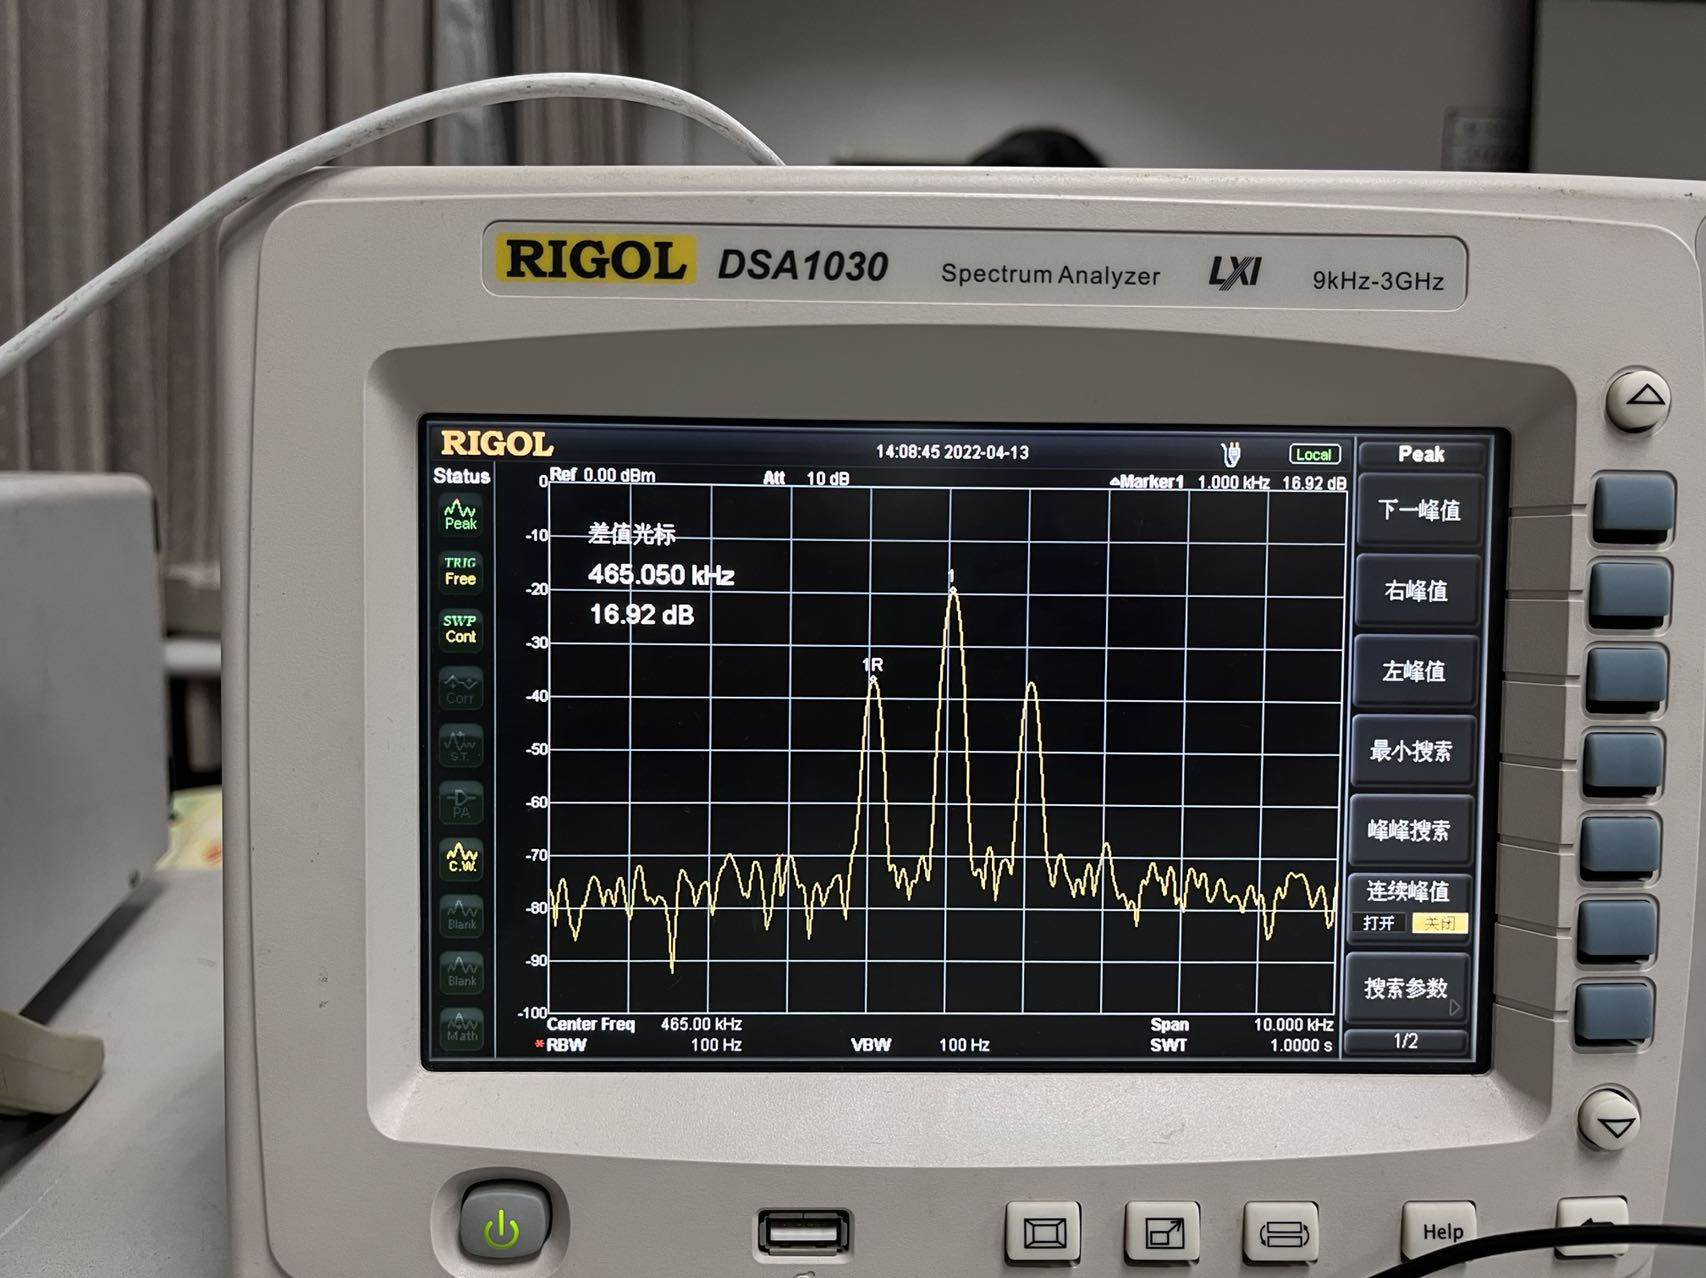
\includegraphics[width = 0.5\textwidth]{lab6/1.jpg}
    \caption{-16.92dBc时相应频域波形}
\end{figure}

此时的调制度$$\mathrm{m}=2 \times 10^{\Delta / 20} \times 100 \%=2 \times 10^{-16.92 / 20} \times 100 \%
=28.15\%$$

第二次测量为边带与载波的幅度差△=-12.14dBc时:
\begin{figure}[H]
    \centering
    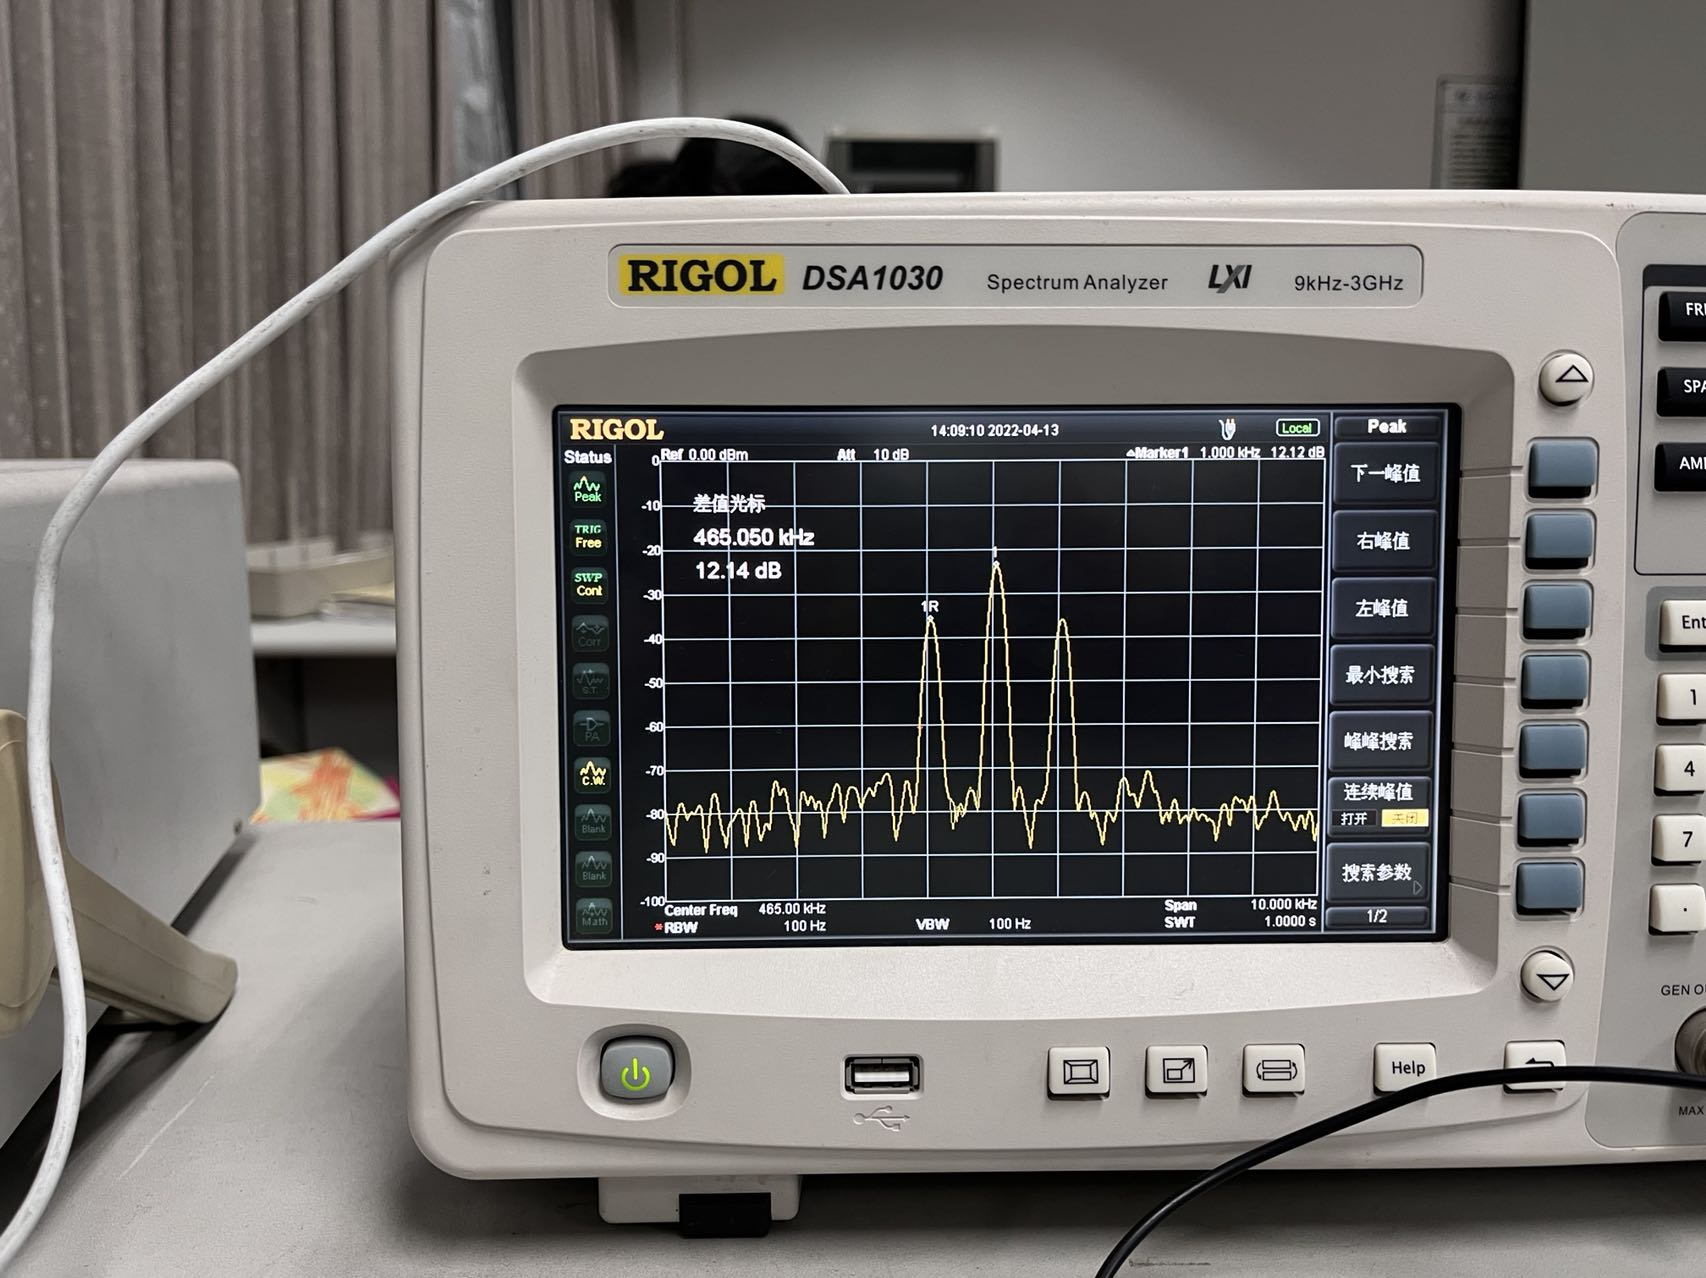
\includegraphics[width = 0.5\textwidth]{lab6/2.jpg}
    \caption{-12.14dBc时相应频域波形}
\end{figure}
此时的调制度$$\mathrm{m}=2 \times 10^{\Delta / 20} \times 100 \%=2 \times 10^{-12.14 / 20} \times 100 \%
=49.43\%$$

第三次测量为边带与载波的幅度差△=-6.10dBc时:
\begin{figure}[H]
    \centering
    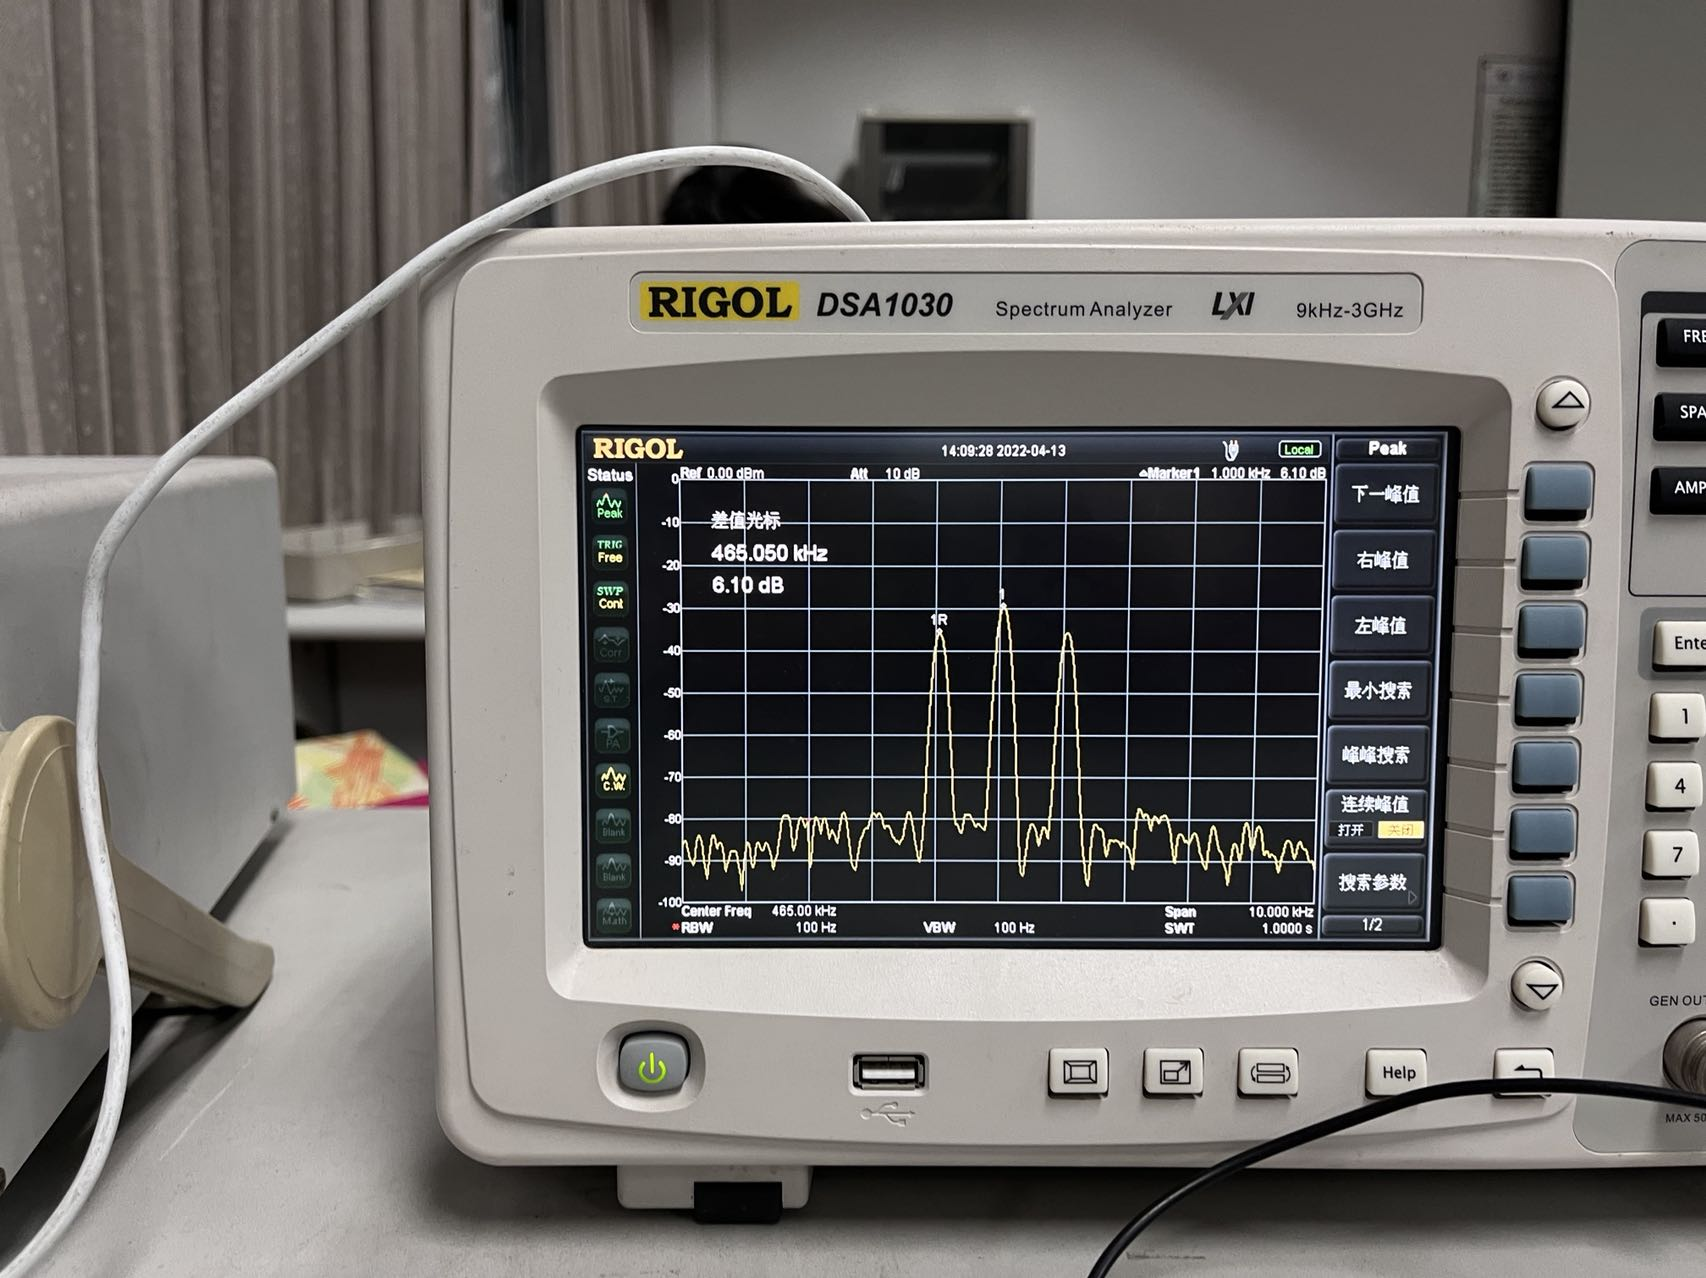
\includegraphics[width = 0.5\textwidth]{lab6/3.jpg}
    \caption{-6.10dBc时相应频域波形}
\end{figure}
此时的调制度$$\mathrm{m}=2 \times 10^{\Delta / 20} \times 100 \%=2 \times 10^{-6.10 / 20} \times 100 \%
=99.09\%$$

通过波形和计算可以知道,当边带与载波的幅度差越小时,调制度越高。

\subsubsection{双边带调制(DSB)}
在普通幅度调制的基础上,调节电位器WR1,同时观察信号频谱,直到频谱中载波分量降
到最低,这就实现抑制载波幅度调制(DSB)。用示波器观察并记录调制输出信号的波形(注
意,将频谱分析仪的电缆从JP4脱开)。

\begin{figure}[H]
    \centering
    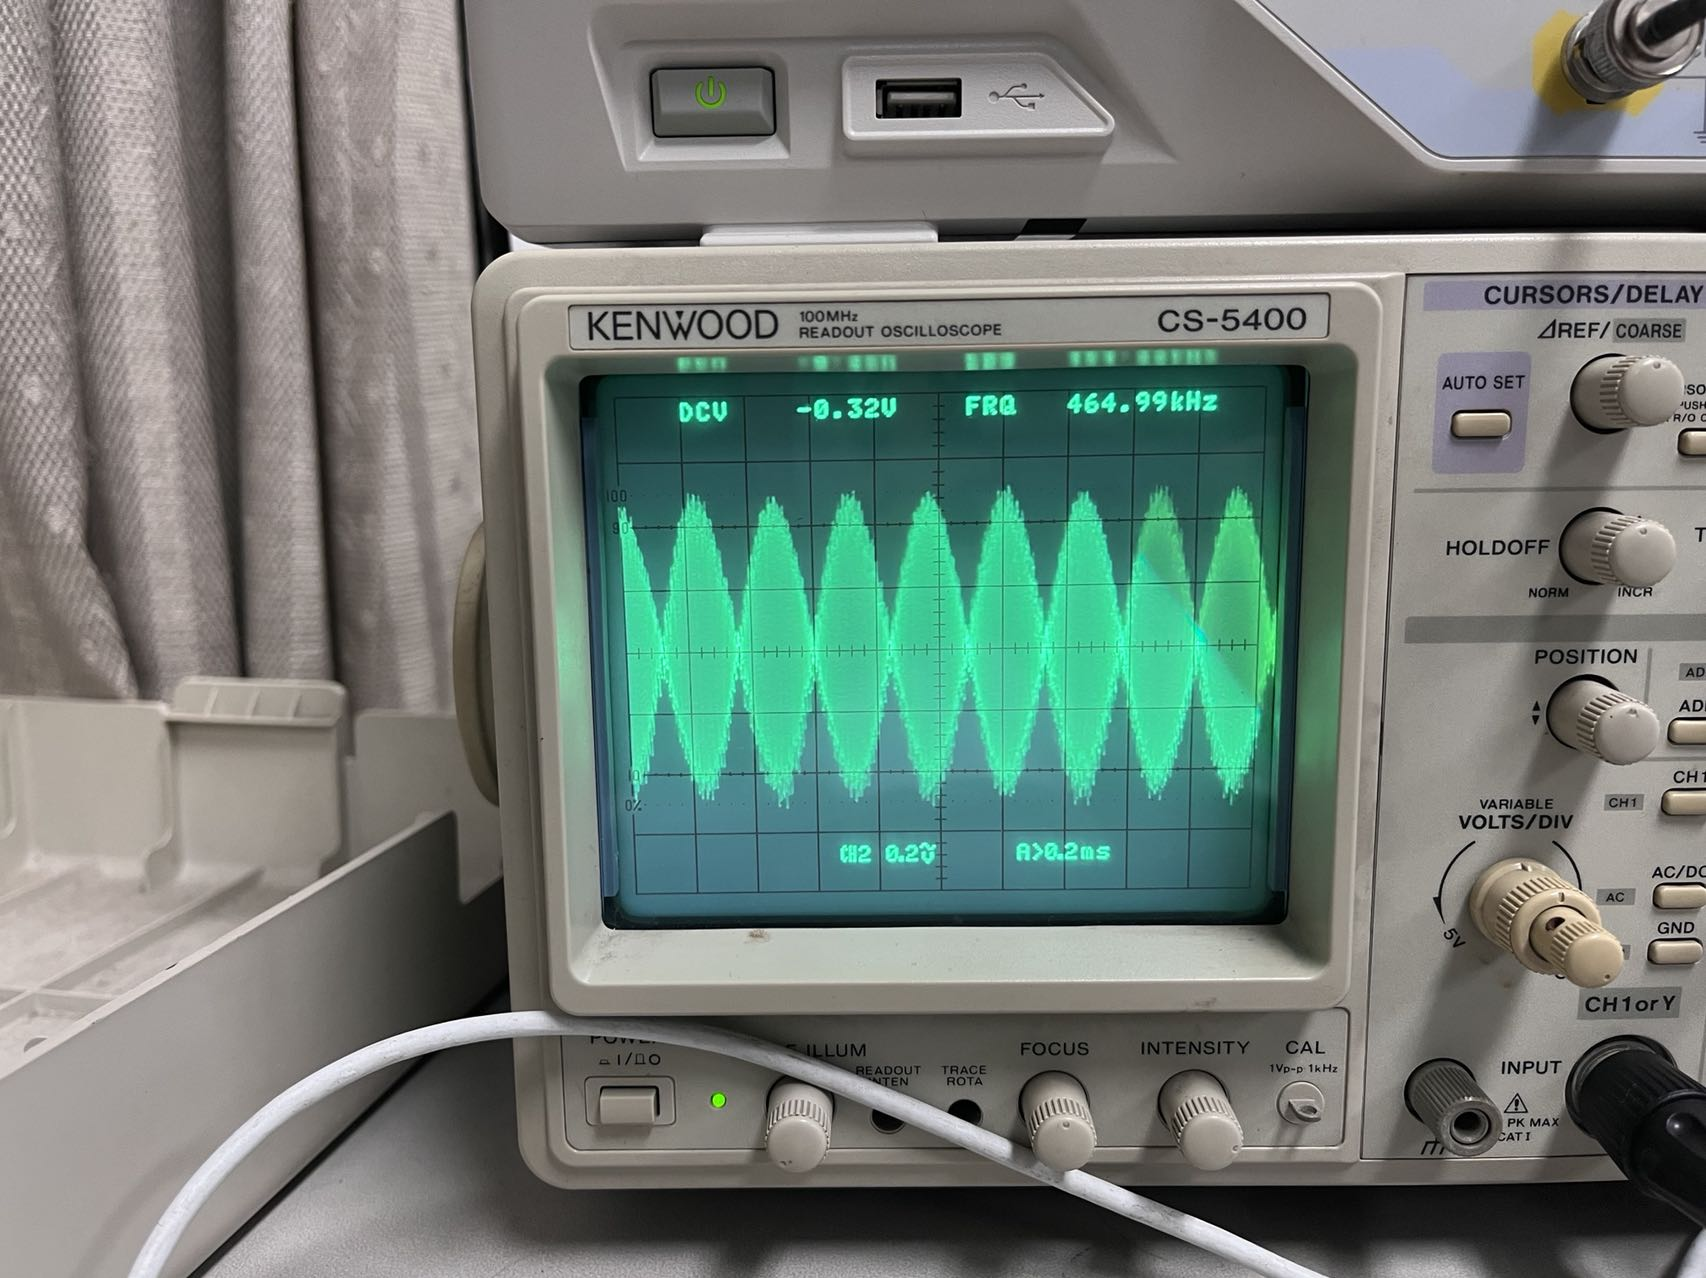
\includegraphics[width = 0.5\textwidth]{lab6/4.jpg}
    \caption{DSB调制输出信号的波形}
\end{figure}

\subsection{同步相干解调实验}
\subsubsection{AM 同步解调}
调整WR1,使调制电路产生AM调制信号,用示波器观测同步解调输出信号。改变JP2端调制
信号幅度,从而改变已调波信号的调制度,观察同步解调输出信号的幅度变化。
\begin{figure}[H]
    \centering
    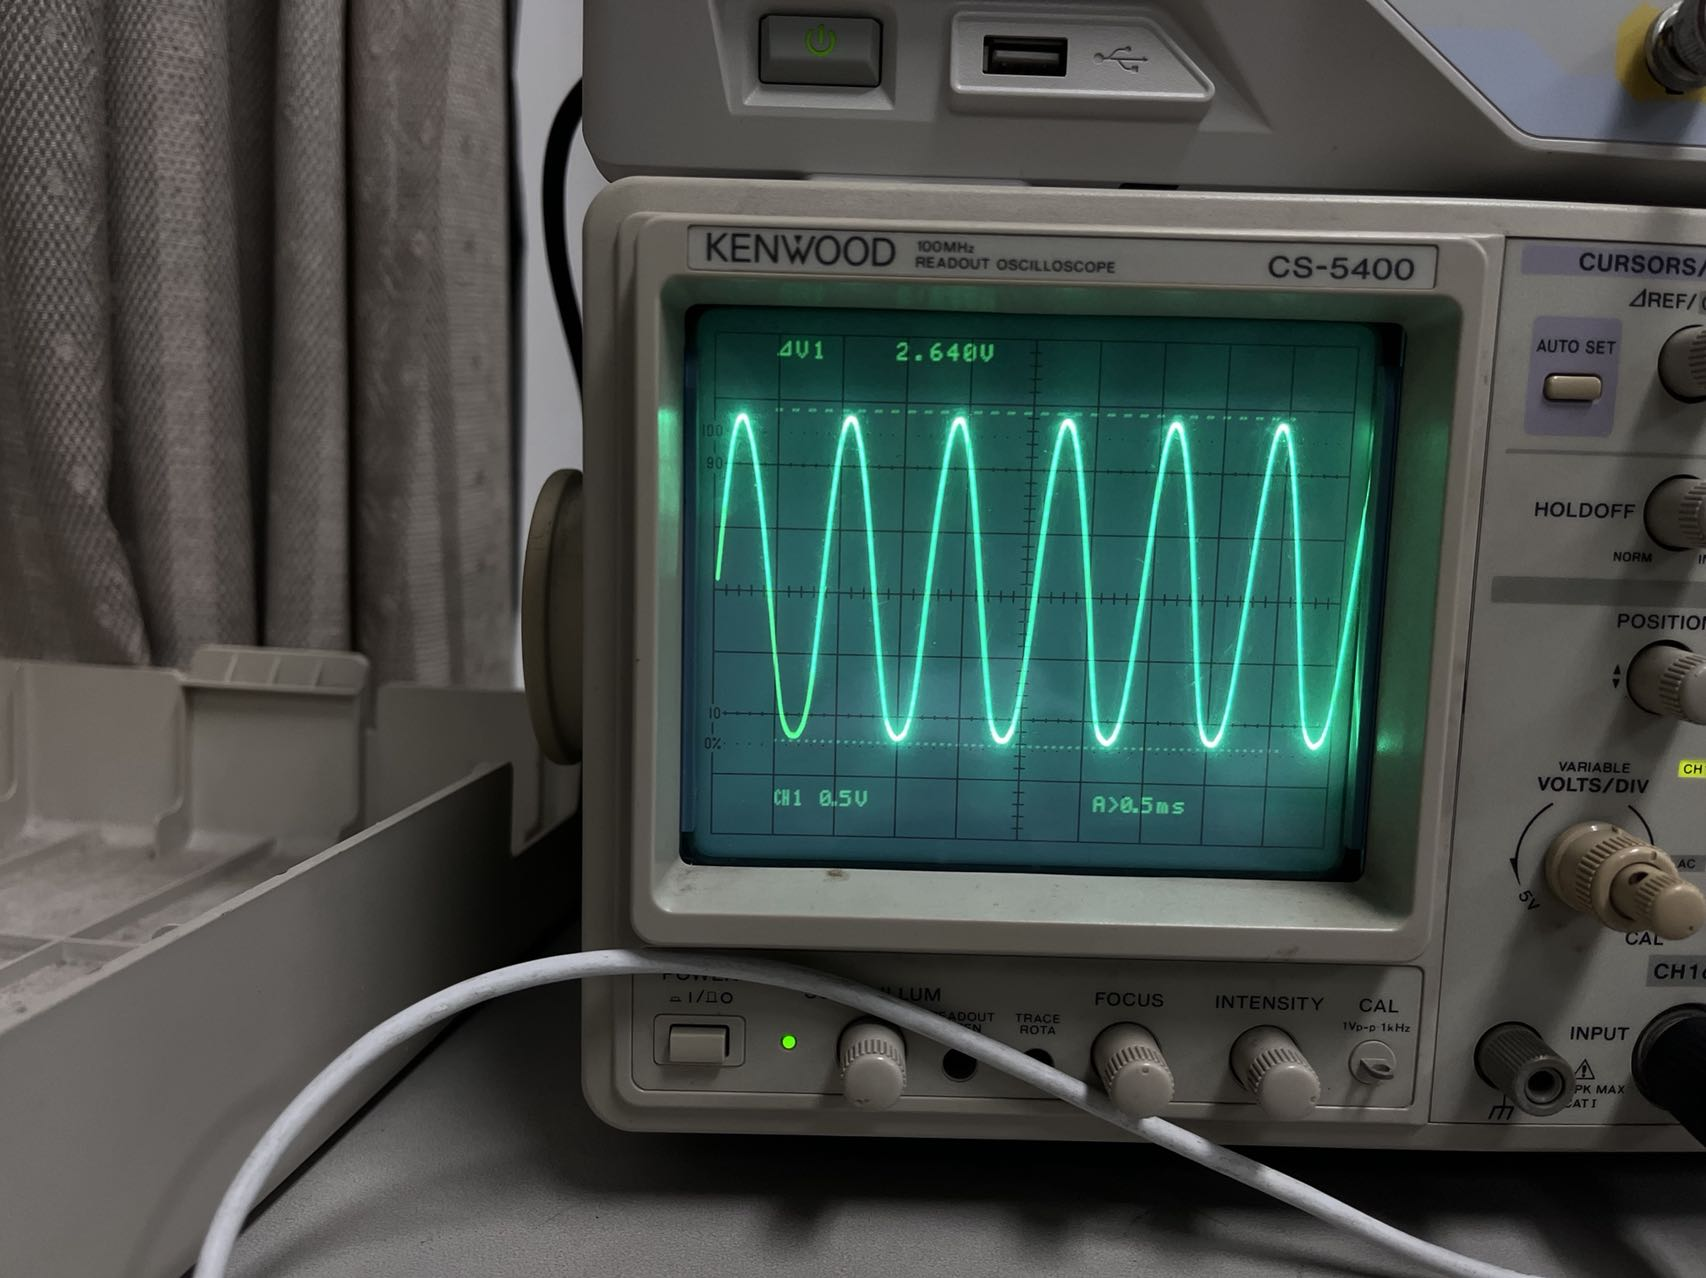
\includegraphics[width = 0.5\textwidth]{lab6/5.jpg}
    \caption{AM 同步解调信号的波形}
\end{figure}

示波器观察到的解调输出波形如上图所示(输入信号0dBm),通过改变调制信号幅度,输出信号幅度相应得到改变:

调制信号:0dBm   解调输出信$号V_{p-p}$=2.64V

调制信号:-12dBm   解调输出信号$V_{p-p}$=0.736V

显然当调制信号值幅度变小时,解调输出信号也相应变小。

\subsubsection{DSB 同步解调}
调整WR1,使调制电路产生DSB调制信号,用示波器观测同步解调输出信号。改变JP2端调
制信号幅度,观察同步解调输出信号的幅度变化。

实验结果类似AM 同步解调类似,当调制信号值幅度变小时,解调输出信号也相应变小。

\subsection{包络检波实验}
由高频信号源从JP4端输入载波频率为465kHz,大小为10dBm(即2Vp-p),调制信号频率
为1kHz的正弦波,调制度为30\%的AM调幅信号。
\subsubsection{惰性
失真}
改变跳线 J1,选择不同的时间常数,用示波器在测试点 TP8观察检波输出信号的惰性
失真情况。
\begin{figure}[H]
    \centering
    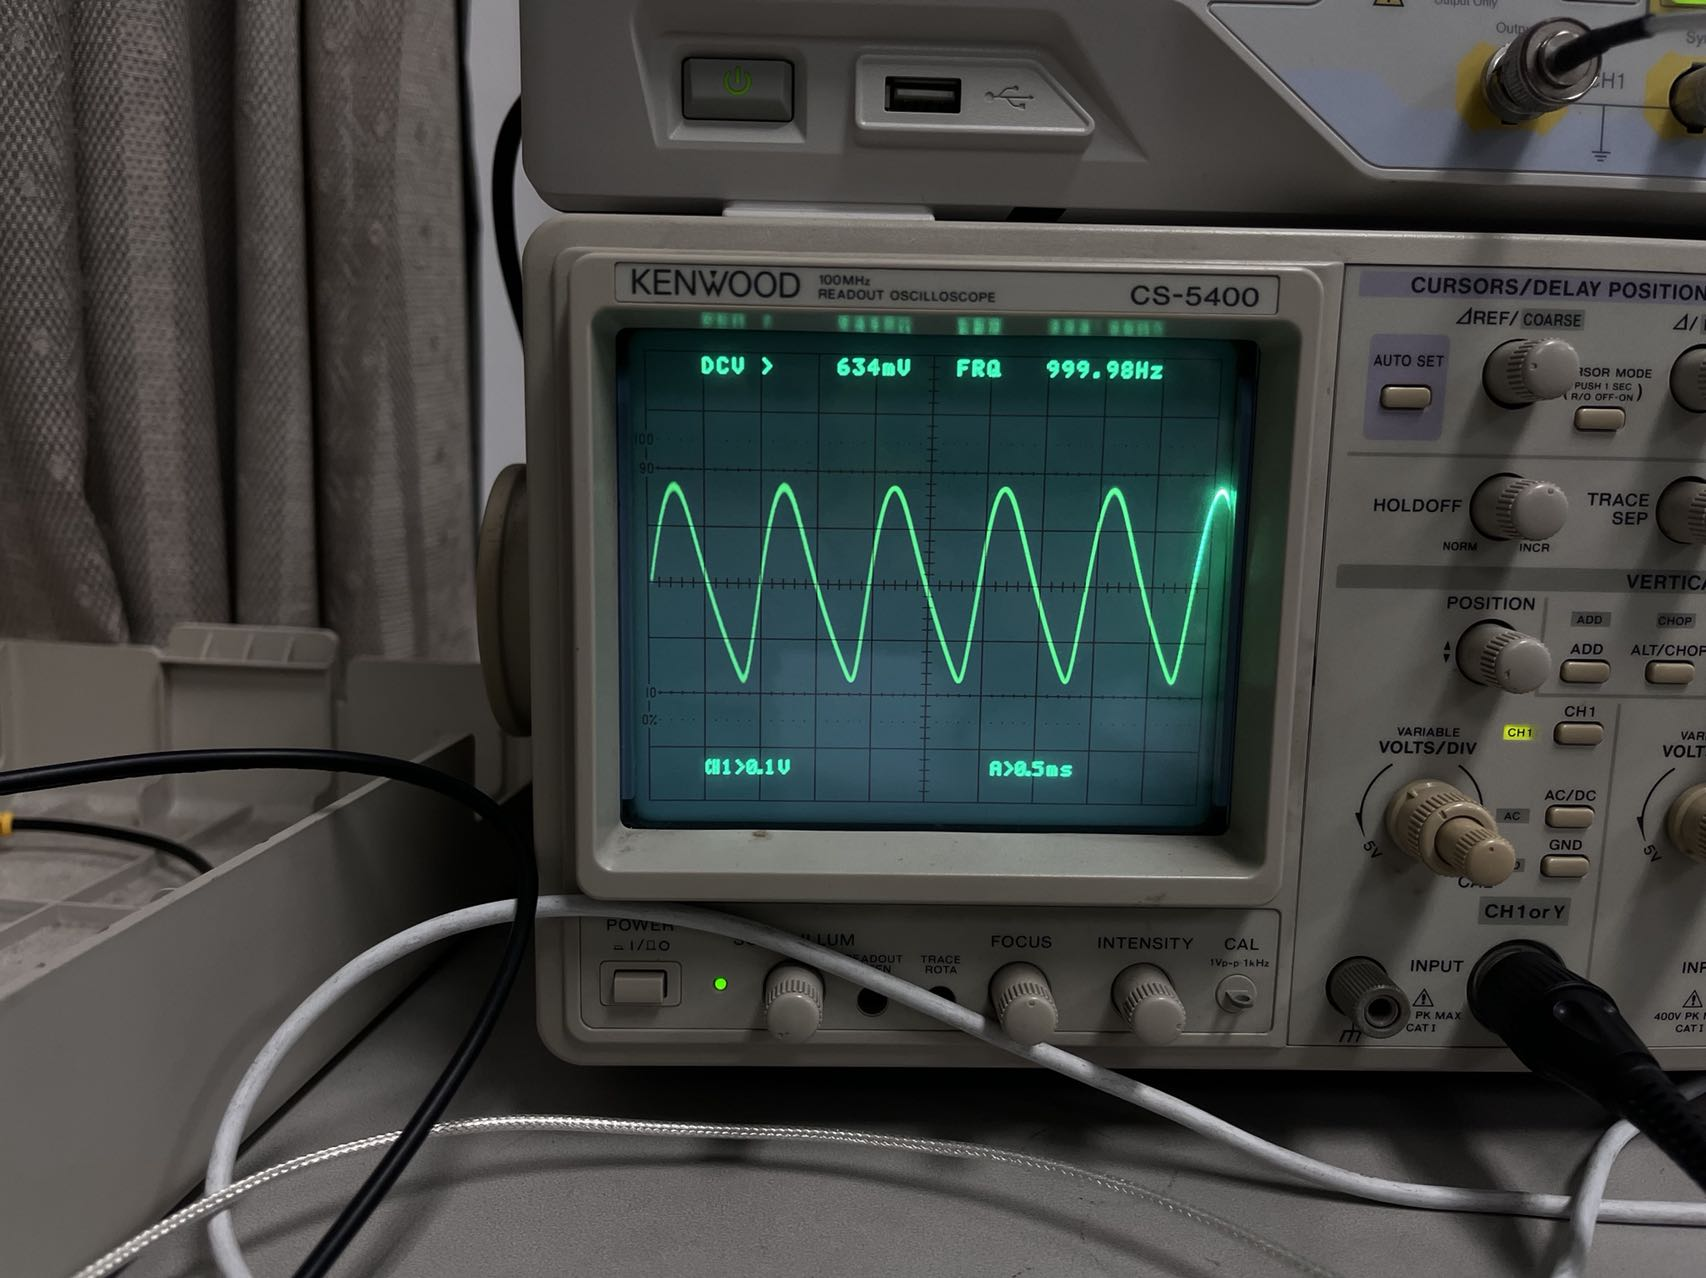
\includegraphics[width = 0.5\textwidth]{lab6/6.jpg}
    \caption{惰性失真情况}
\end{figure}

\subsubsection{负峰
切割失真}
改变跳线 J2,选择不同的交流阻抗,用示波器在测试点 TP10观察检波输出信号的负峰
切割失真情况。
\begin{figure}[H]
    \centering
    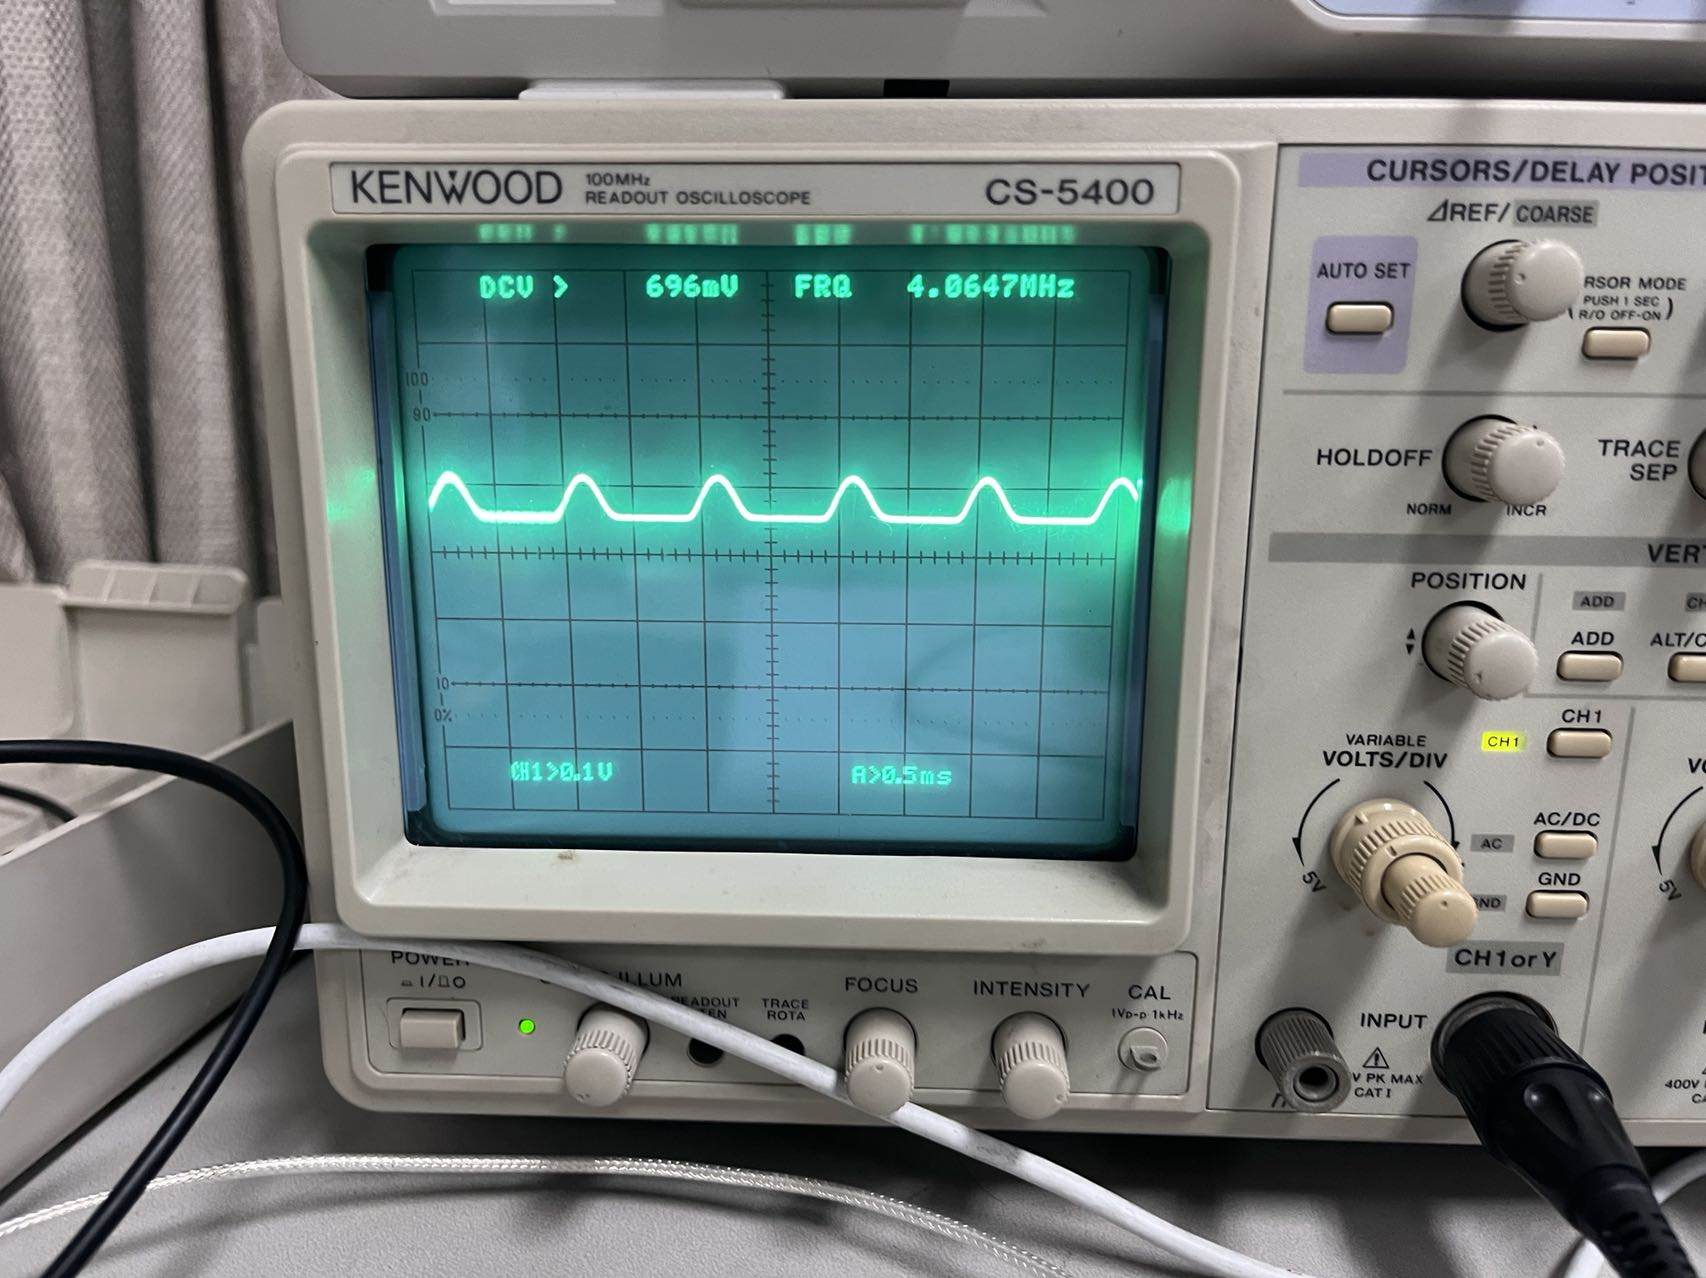
\includegraphics[width = 0.5\textwidth]{lab6/7.jpg}
    \caption{负峰
    切割失真}
\end{figure}

\subsubsection{何时出现失
真}
在无失真的情况下,改变输入信号的调制度,观察对输出信号的影响(何时出现失
真)?
\begin{figure}[H]
    \centering
    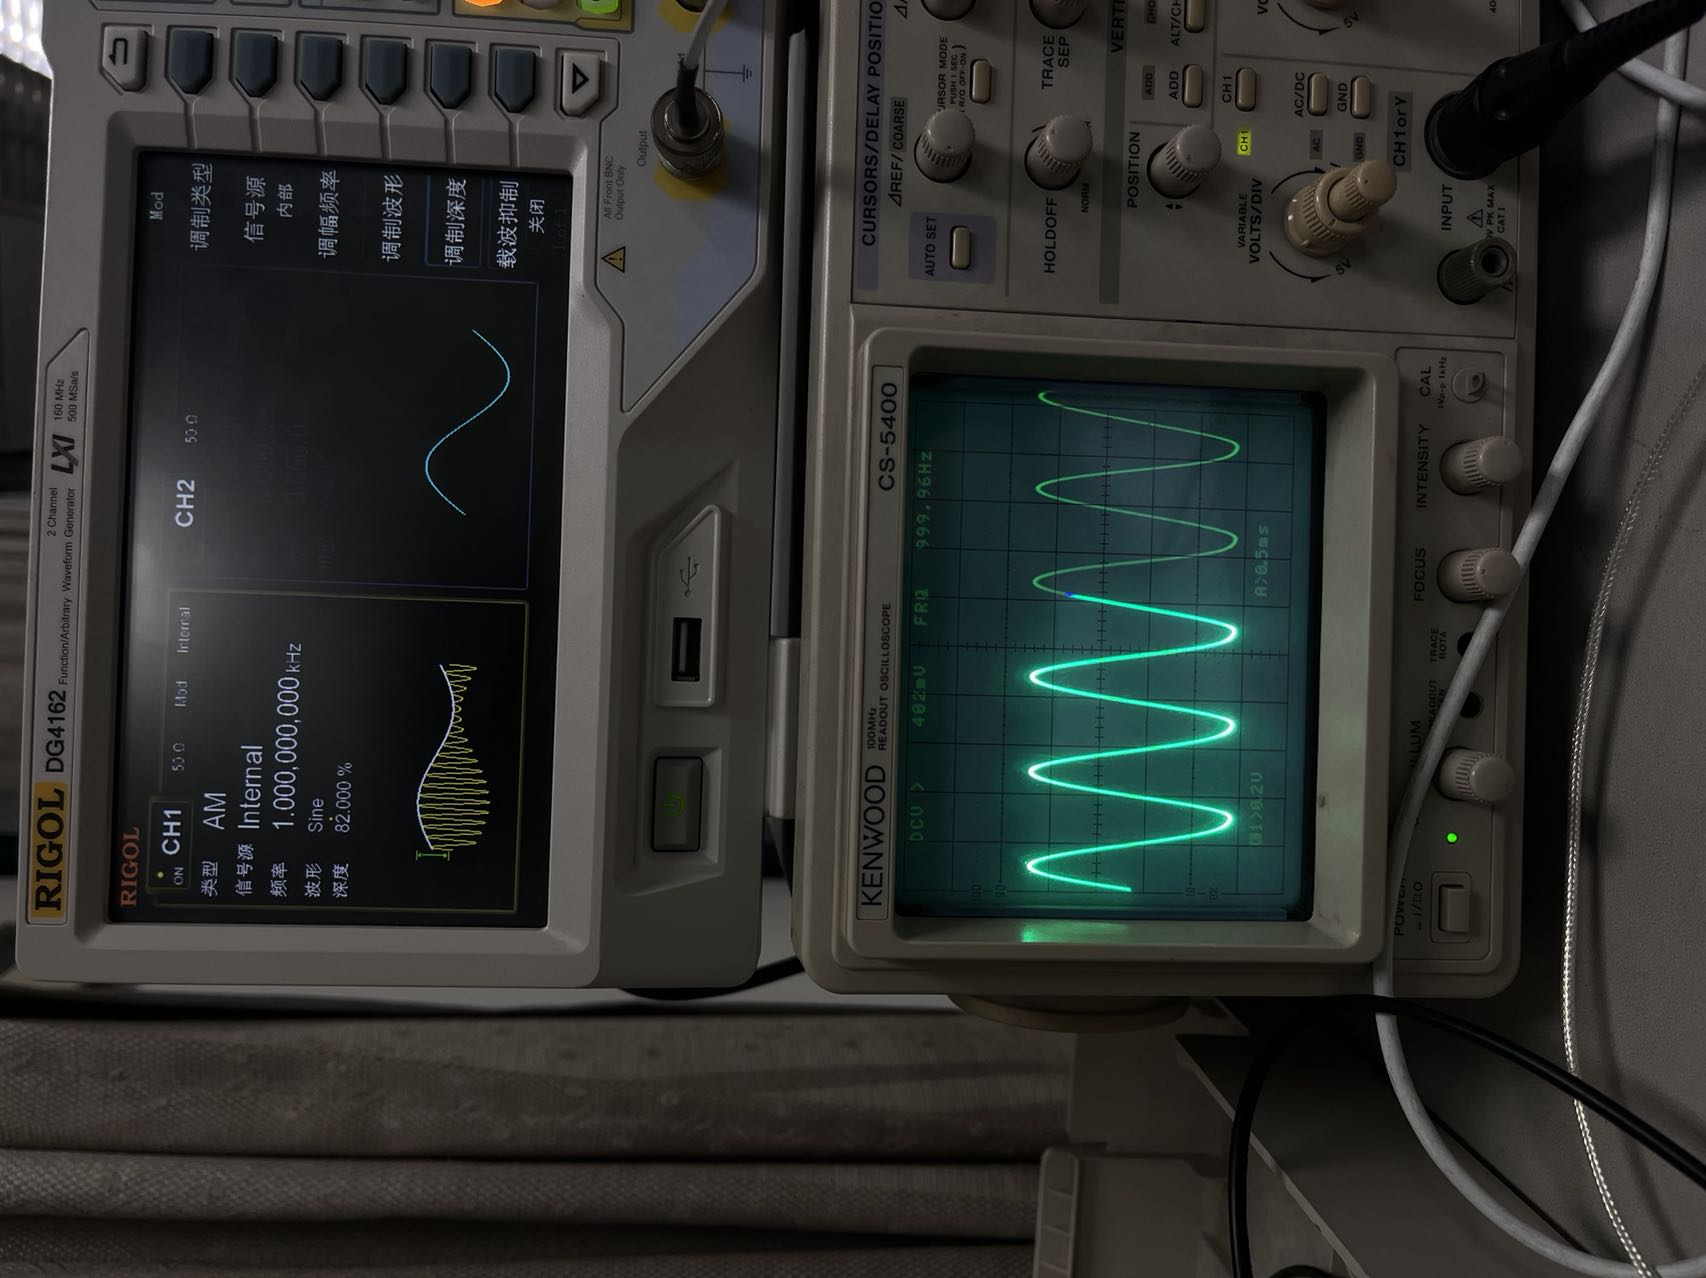
\includegraphics[width = 0.5\textwidth,angle=270]{lab6/8.jpg}
    \caption{何时出现失
    真}
    
\end{figure}

经过测试,发现调制度为82\%左右的时候出现失真。

\section{思考题}
(1) AM、DSB 调制有何区别,它们分别是如何实现的?

AM调制是普通调幅,使载波的振幅按照所需传送信号的变化规律而变化,但频率保持不变。DSB是双边带抑制载波调幅。是通过幅度调制(AM)使得频率关于载波频率对称分布,且将载波电平降低到最低程度。


(2) 已调波信号的调制度与什么因素有关系?

$m_{a}=\frac{k V_{\Omega m}}{V_{c m}}$ 是调幅系数,也称调制度。

因此与k,$V_{\Omega m},V_{c m}$有关,k是由电路决定的常量,$V_{\Omega m}$是调制信号幅度峰值,$V_{c m}$是载波信号的幅度峰值。


(3) 包络检波输出信号产生惰性失真和负峰切割失真的原因分别是什么?如何改善失真
情况?

惰性失真原因:当RC时间常数过大,电容C通过电阻R放电的速度过慢,使得电容器
上的电压变化跟不上信号包络的下降速度。在输入信号的好几个周期内,二极管都没有导通,
则输出电压没有反应输入信号的包络变化,出现失真。

如何改善:使电容C通过电
阻R放电的速度不能小于输入信号包络下降的速度:

即:$R C \leq \frac{\sqrt{1-m_{a}^{2}}}{\Omega m_{a}}$

负峰切割失真的原因:在接收机中, 检波器后面接音频放大器。如图所示, 假设 检波器下级电路的输入阻抗为 $\mathrm{R}_{\mathrm{L}}$, 那么检波器的直流负载为 $\mathrm{R}$, 交流负载为 $R / / R_{L}$ 。检波器输 出的交流、直流电流幅度的比值为:
$$
m_{a} \frac{R}{R / / R_{L}}=m_{a} \frac{R+R_{L}}{R_{L}}
$$
当这个比值大于 1 时, 检波电流中的交流量大于直流量, 电流出现负值。因为二极管是单 向导电的, 电流不可能为负值, 只能为零, 所以检波输出电压的负峰值被削平, 也就是产生 负峰切割失真。

如何改善:使上述比值小于1。


(4) DSB 调制信号是否可以通过包络检波方式进行解调?

不可以。
\end{document}